\section{Detailed Performance Results}
\label{Se:perf}

%
We depict the detailed performance results in the following Figures \ref{Fi:case1th}-\ref{Fi:case4th}, where for each benchmark we plot the results when increasing the size of the workload while fixing the number of threads (on the left), and when varying the number of threads (on the right).
Each plot presents a two column diagram, corresponding to STM and corrective synchronization (left/black and right/gray, respectively), which indicates the relative gain thanks to these approaches in comparison with lock-based synchronization. Indeed, the lock-based solution is overly conservative, yielding roughly a linear trend line of decrease in performance as either workload size or the number of threads increases.

\newcommand\mywidth{0.5 \textwidth}
\begin{figure*}
  \rotatebox{90}{\scriptsize Tomcat {\sf ApplicationContext}}
  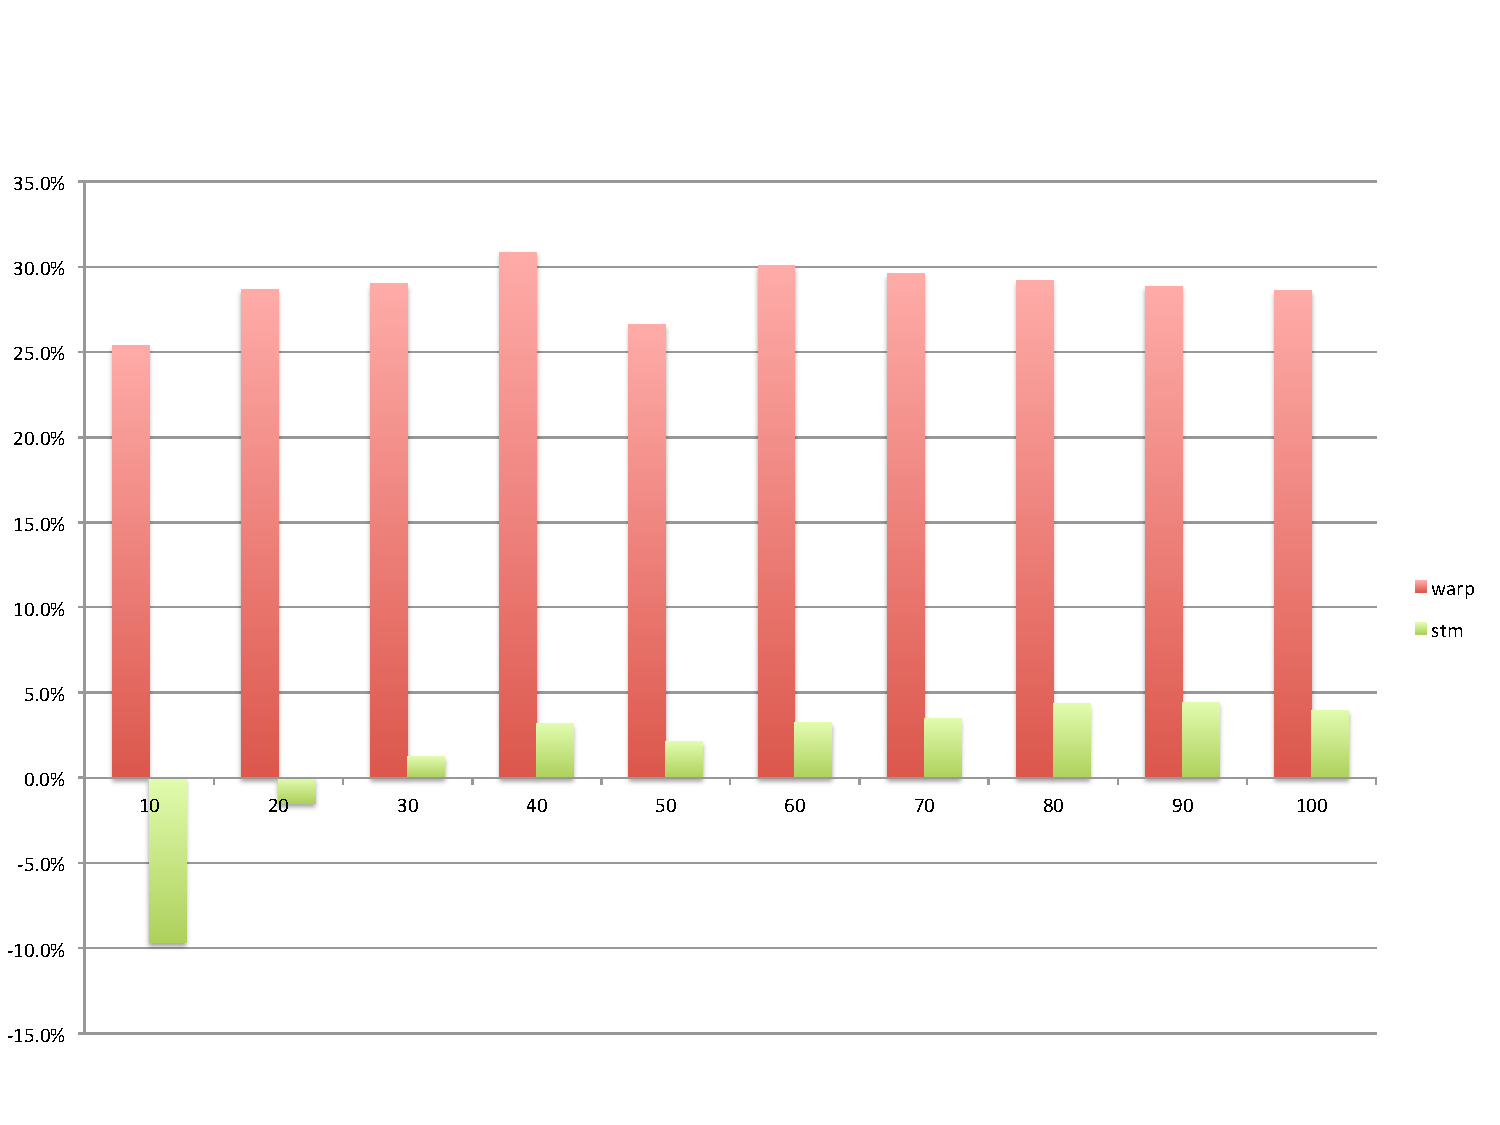
\includegraphics[width=\mywidth]{../../eval/32threads/case1it.pdf}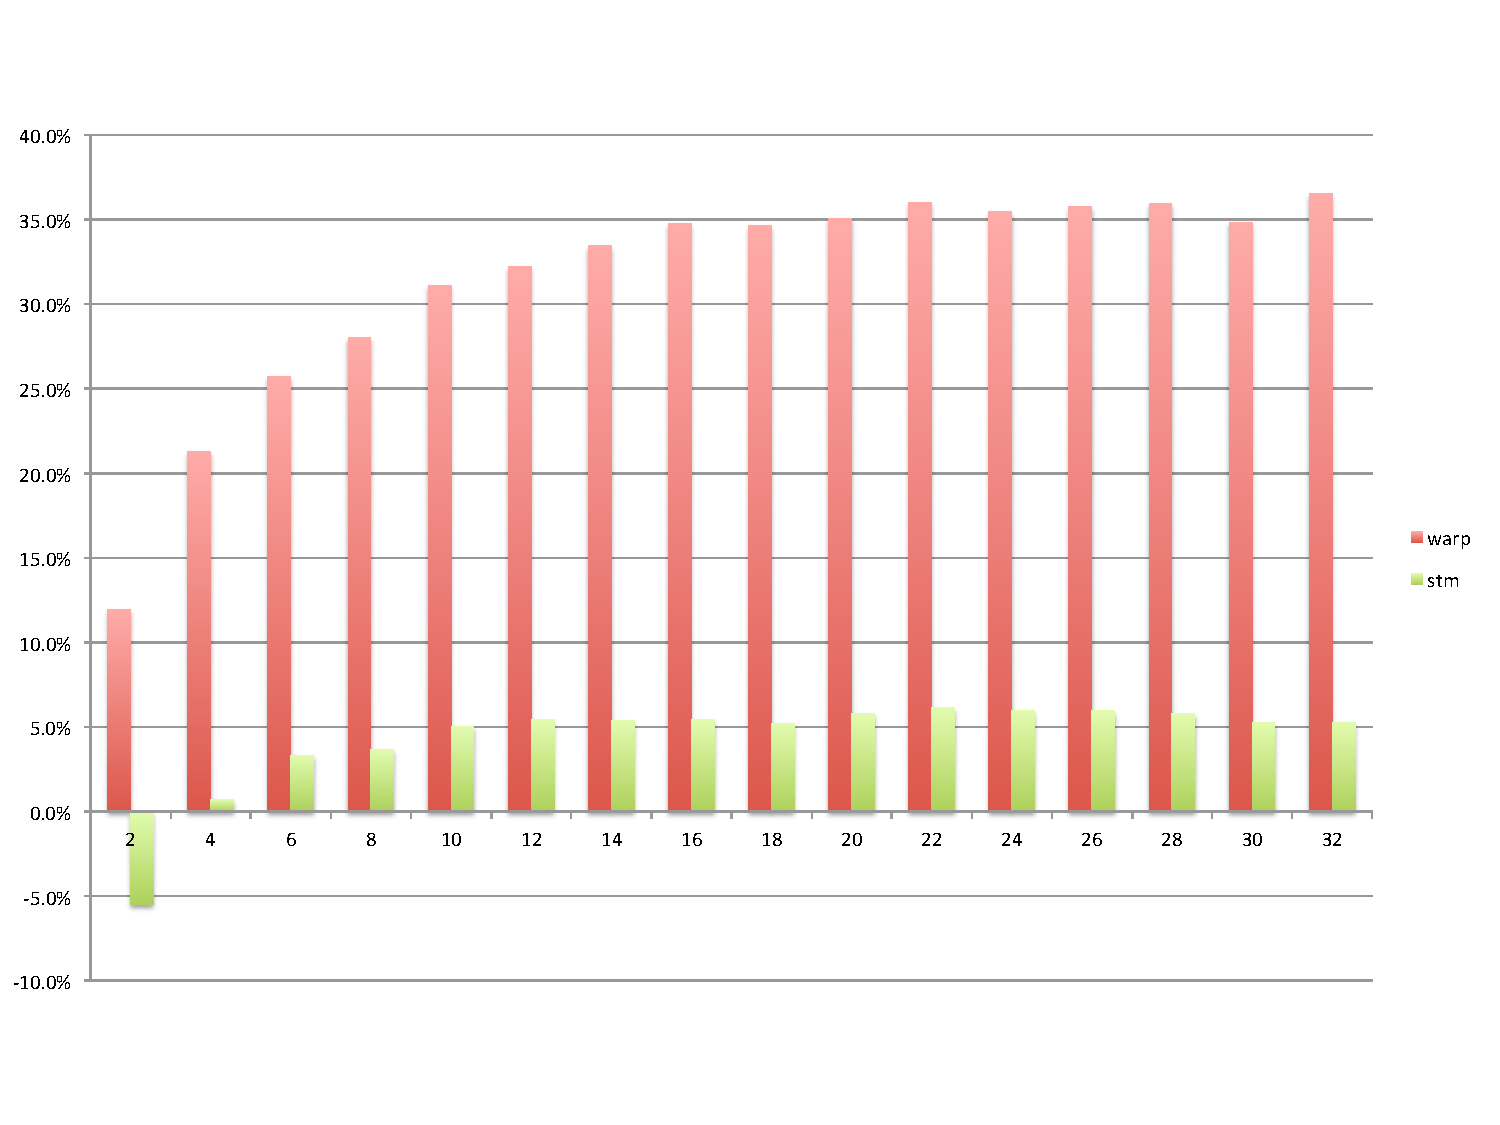
\includegraphics[width=\mywidth]{../../eval/32threads/case1th.pdf}\\
  \rotatebox{90}{\scriptsize dyuproject {\sf StdConvertorCache}}
  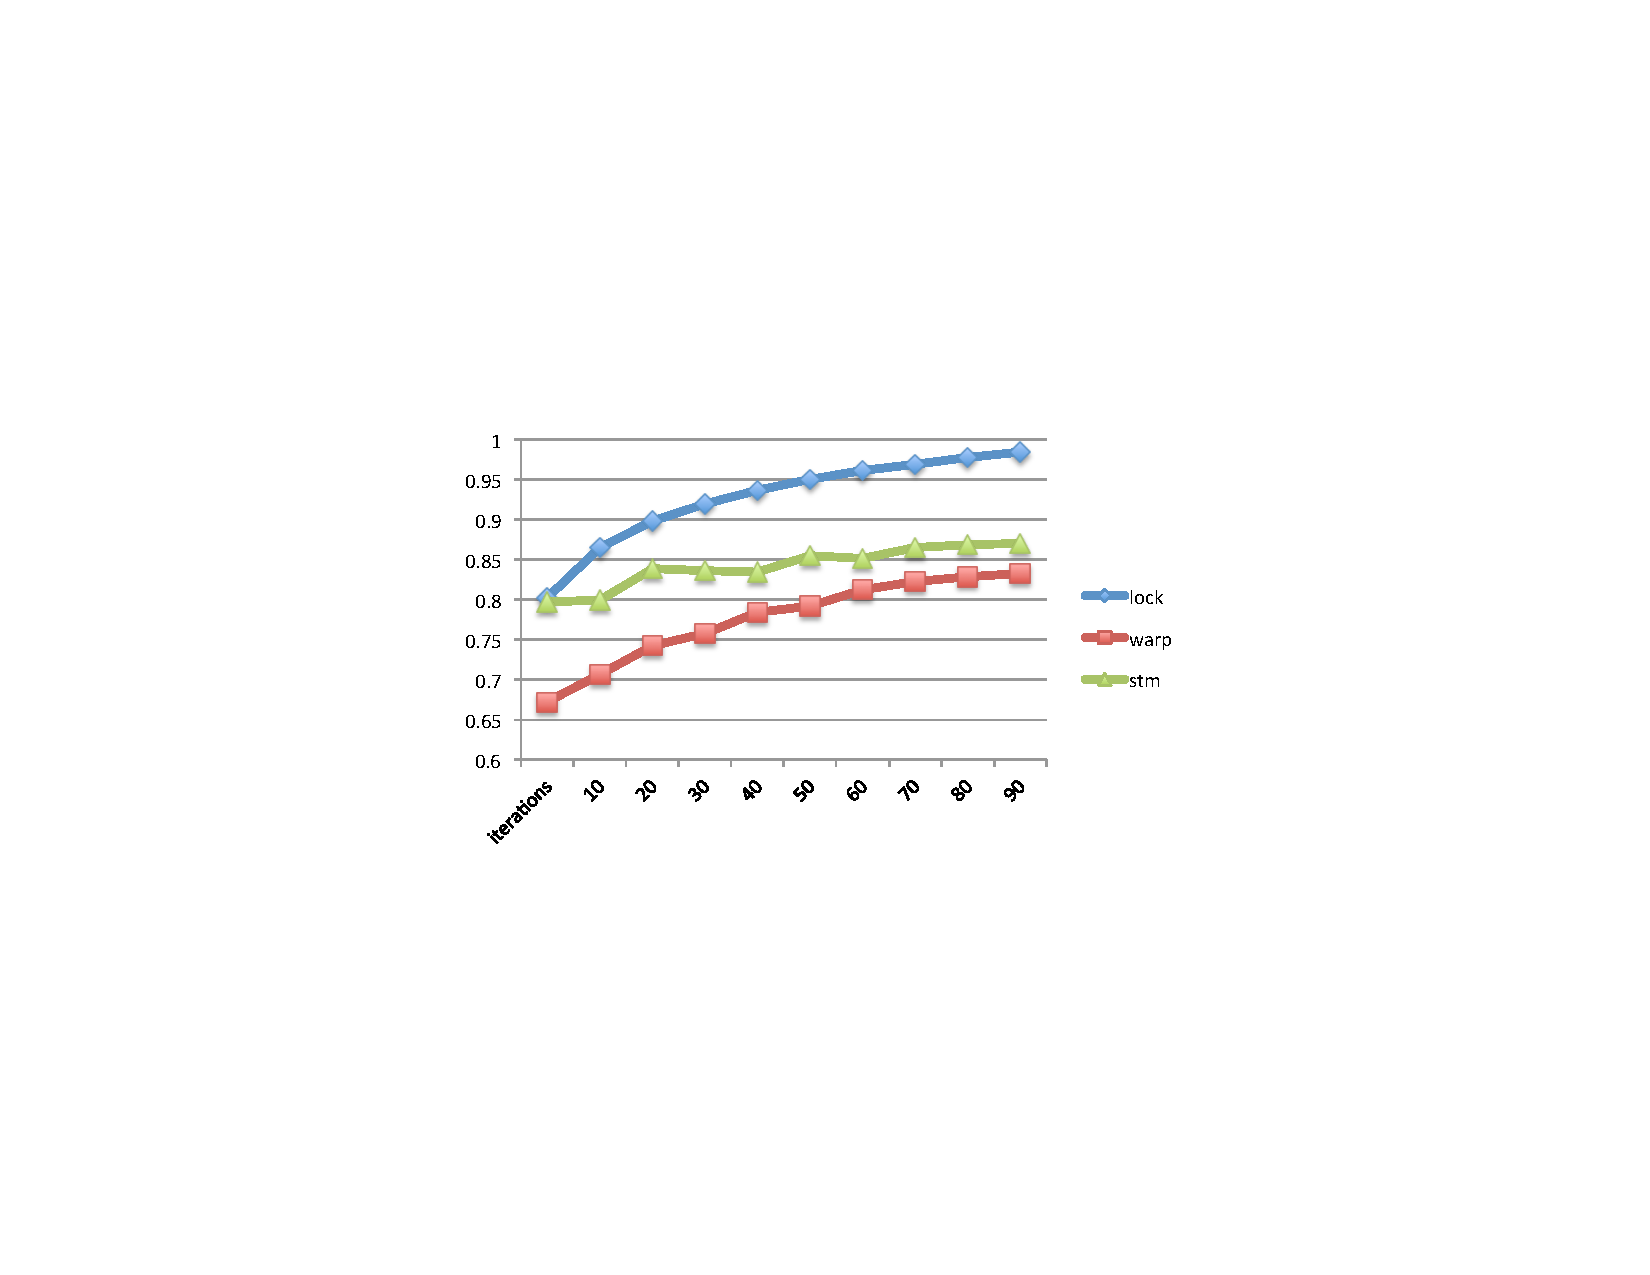
\includegraphics[width=\mywidth]{../../eval/32threads/case2it.pdf}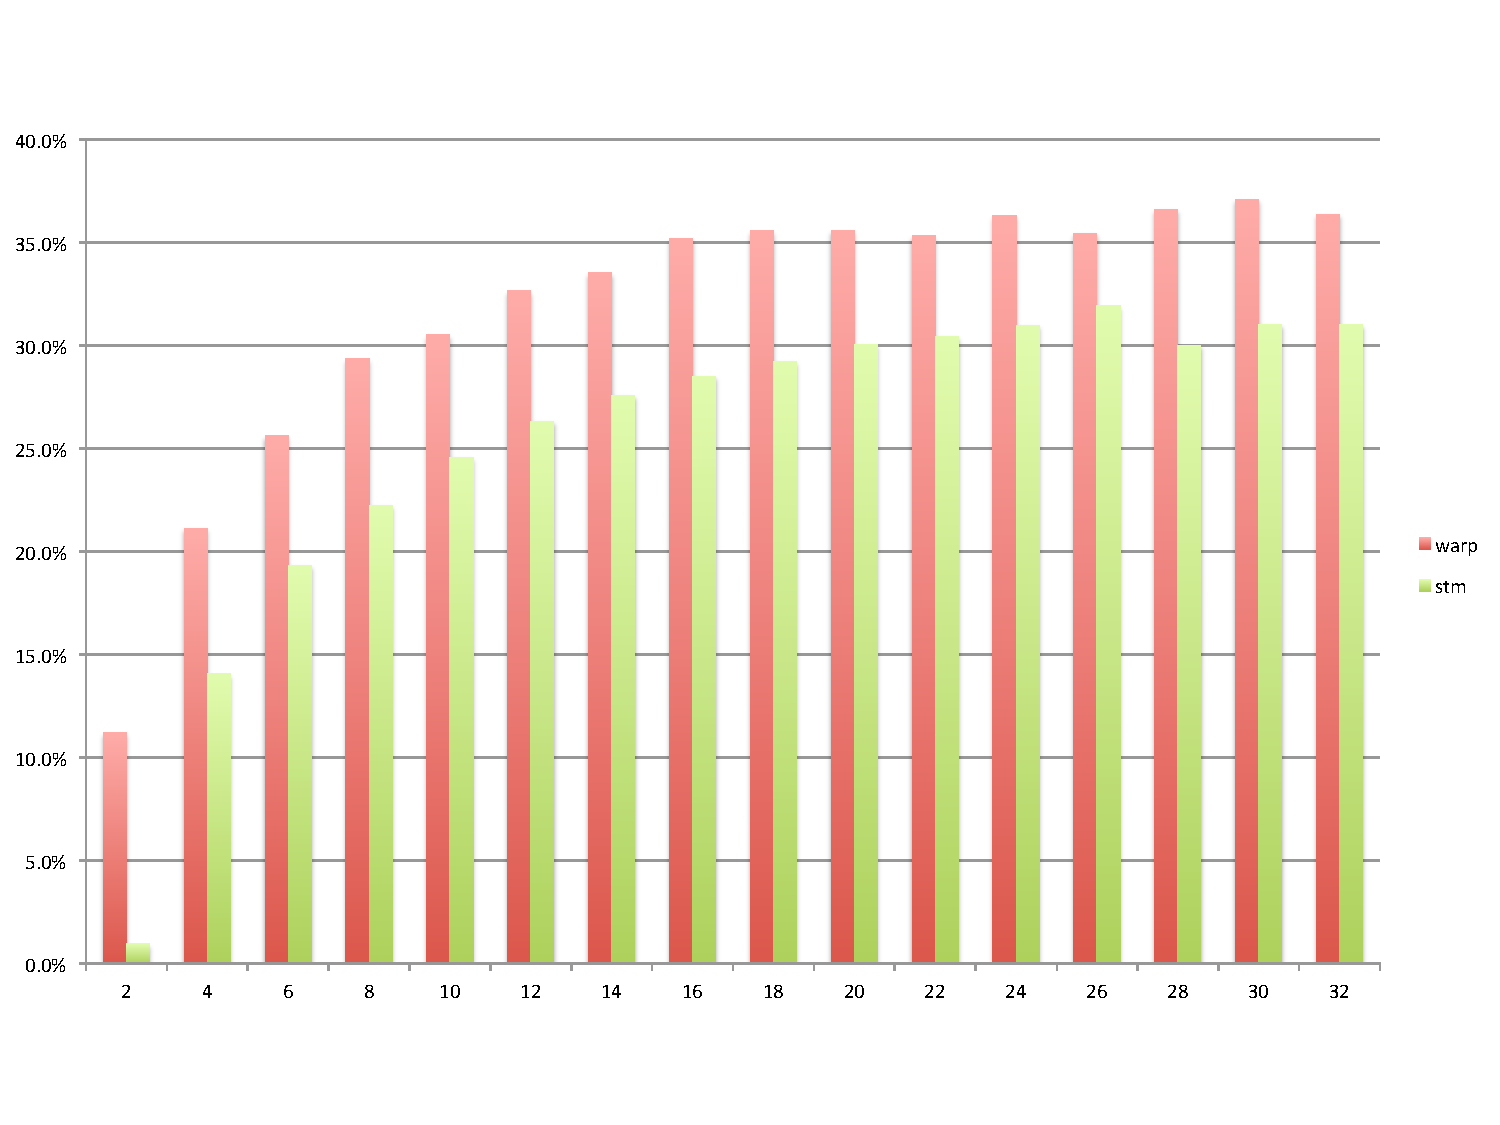
\includegraphics[width=\mywidth]{../../eval/32threads/case2th.pdf}\\
  \rotatebox{90}{Tomcat {\sf ApplicationContext}}
  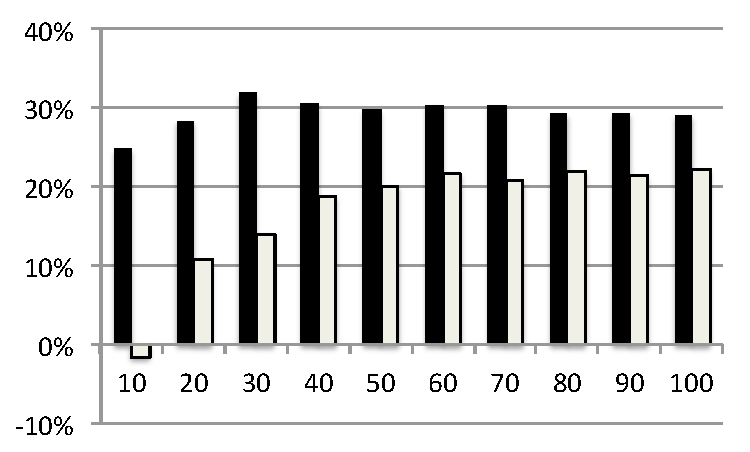
\includegraphics[width=\mywidth]{../../eval/32threads/case3it.pdf}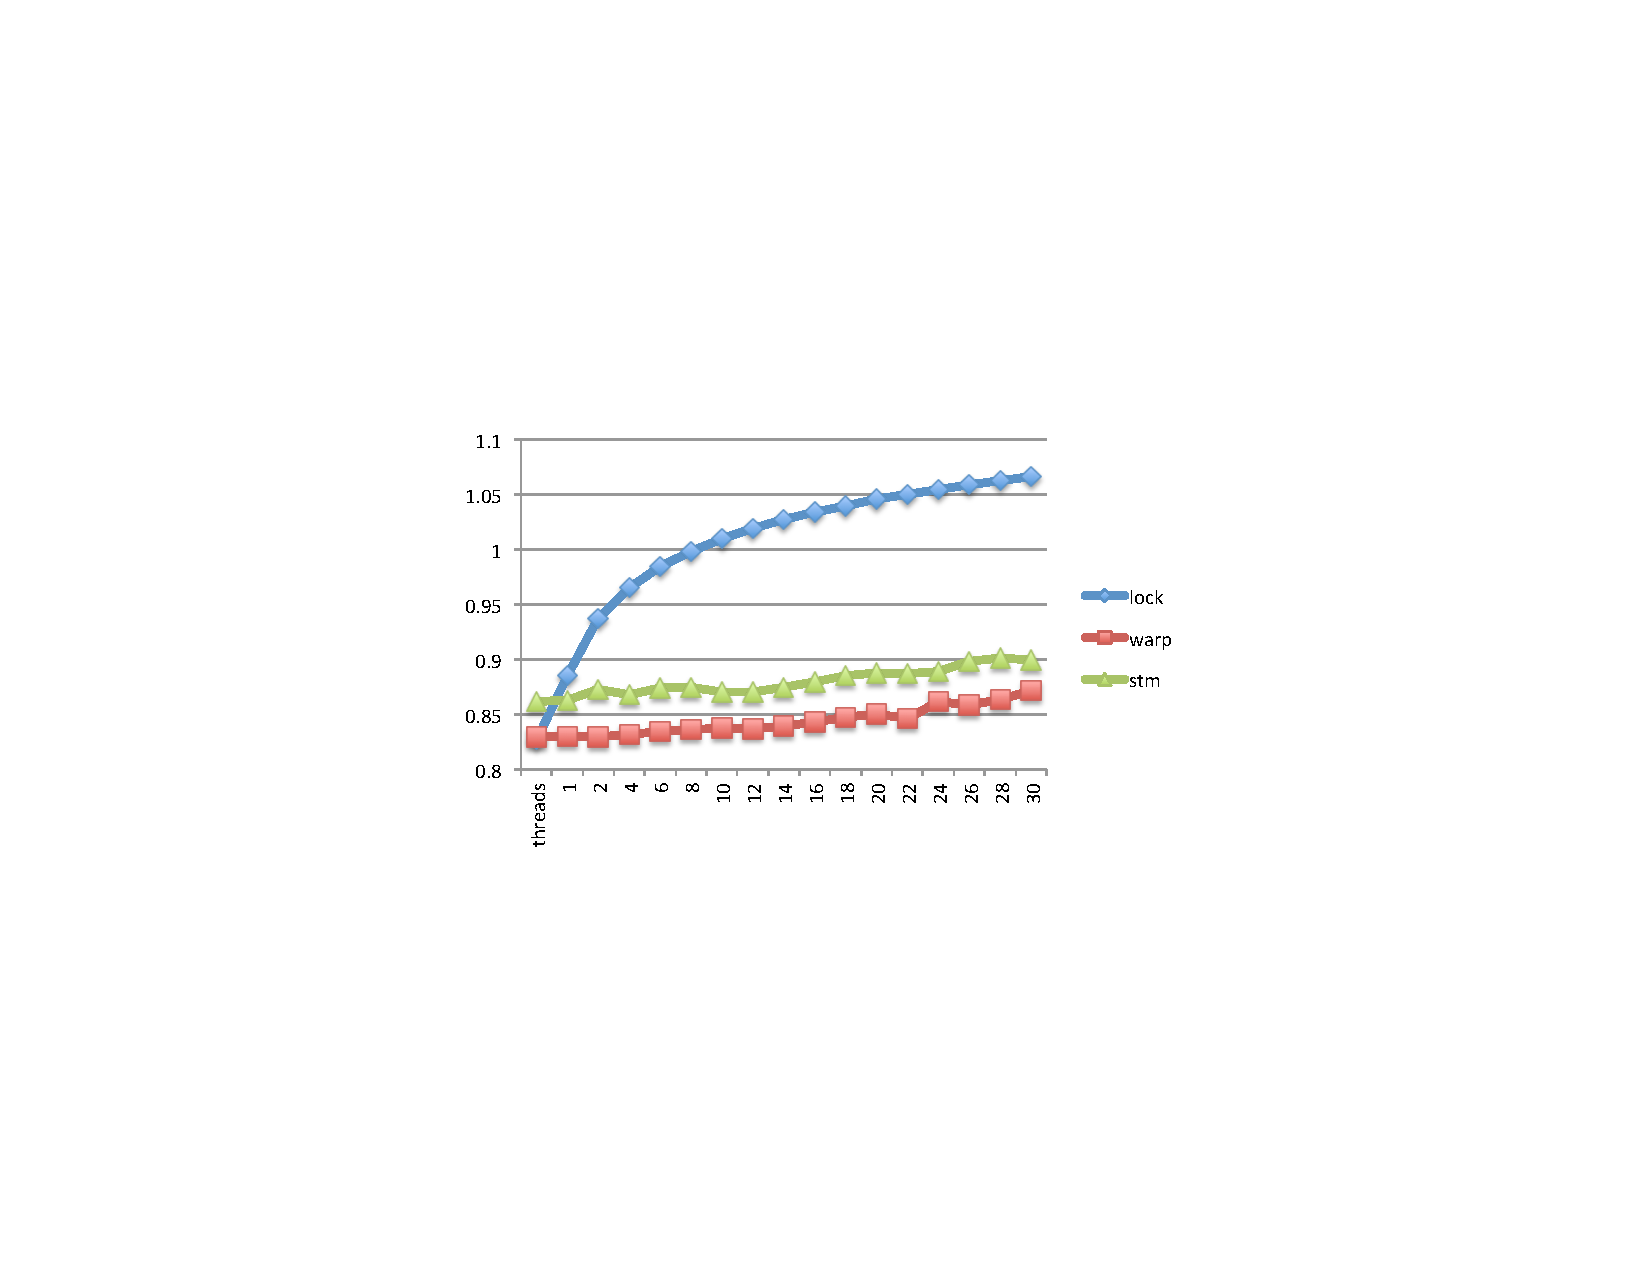
\includegraphics[width=\mywidth]{../../eval/32threads/case3th.pdf}
\end{figure*}
\vspace{-1cm}
\begin{figure*}
  \rotatebox{90}{Tomcat {\sf ApplicationContext}}
  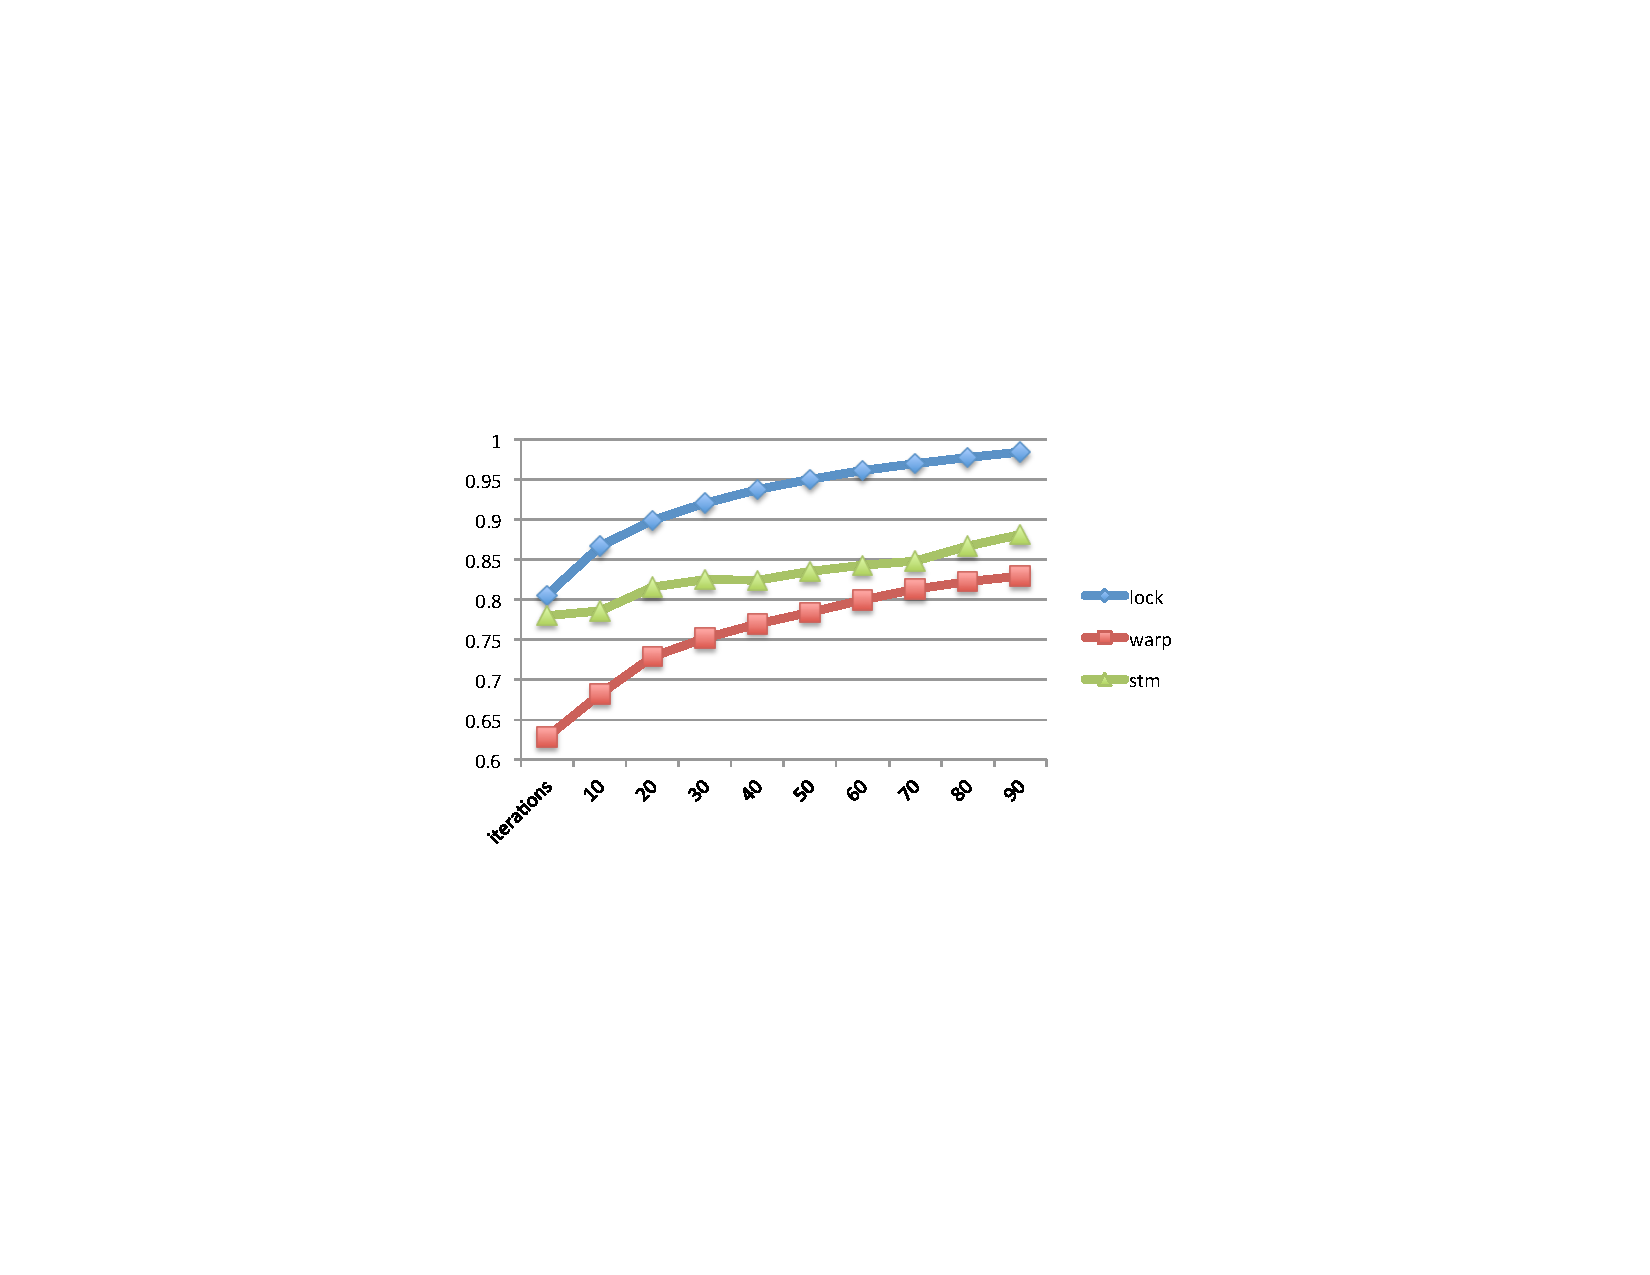
\includegraphics[width=\mywidth]{../../eval/32threads/case4it.pdf}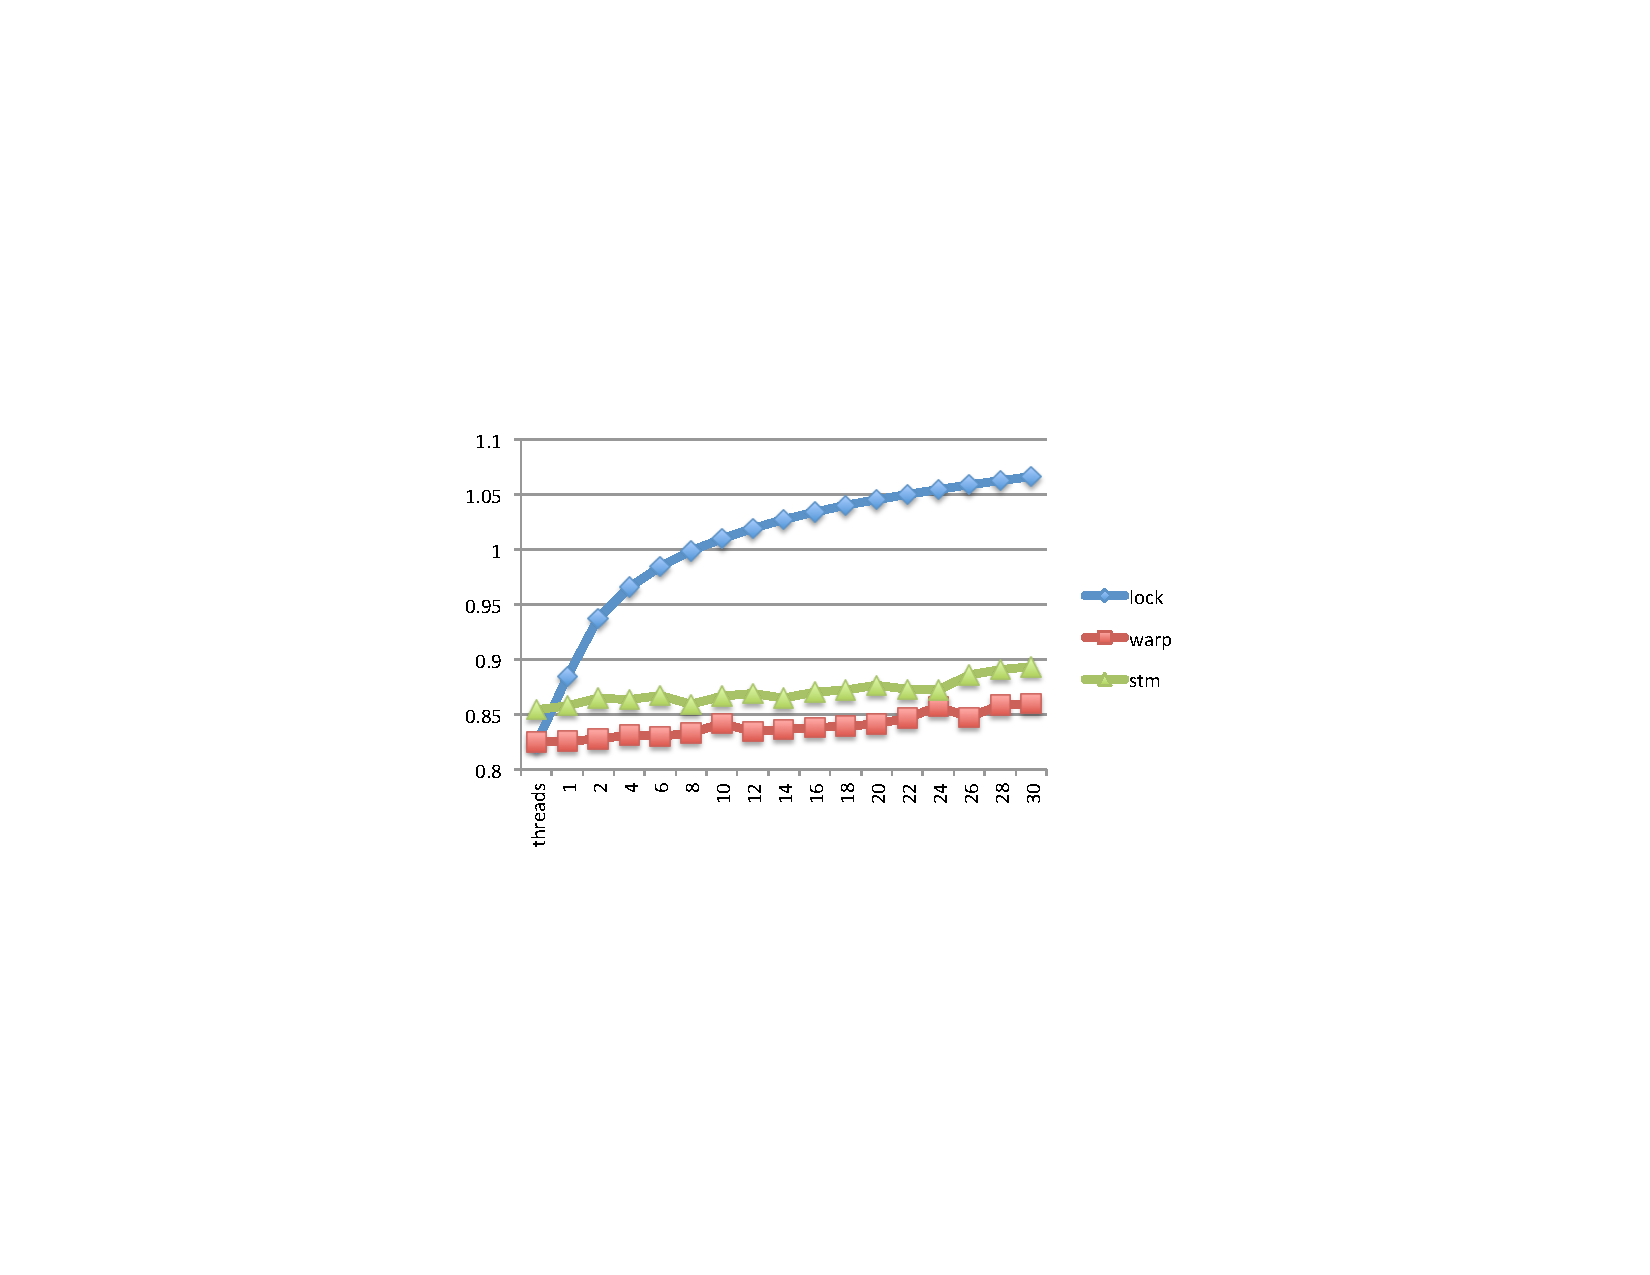
\includegraphics[width=\mywidth]{../../eval/32threads/case4th.pdf}
\end{figure*}

  \vspace{-0.8cm}\caption{\label{Fi:case1th}Apache(l: workload; r: conc)\vspace{-0.2cm}}
  \vspace{-0.8cm}\caption{\label{Fi:case2th} 
    (l: workload; r: conc)\vspace{-0.2cm}}
  \vspace{-0.8cm}\caption{\label{Fi:case3th}Flexive {\sf FxValueRendererFactory} 
			(l: workload; r: conc)\vspace{-0.2cm}}
  \vspace{-0.8cm}\caption{\label{Fi:case4th}Gridkit {\sf ReflectionPofSerializer}
    (l: workload; r: conc)\vspace{-0.2cm}}

  
%	
%	\begin{minipage}{0.3 \textwidth}
%		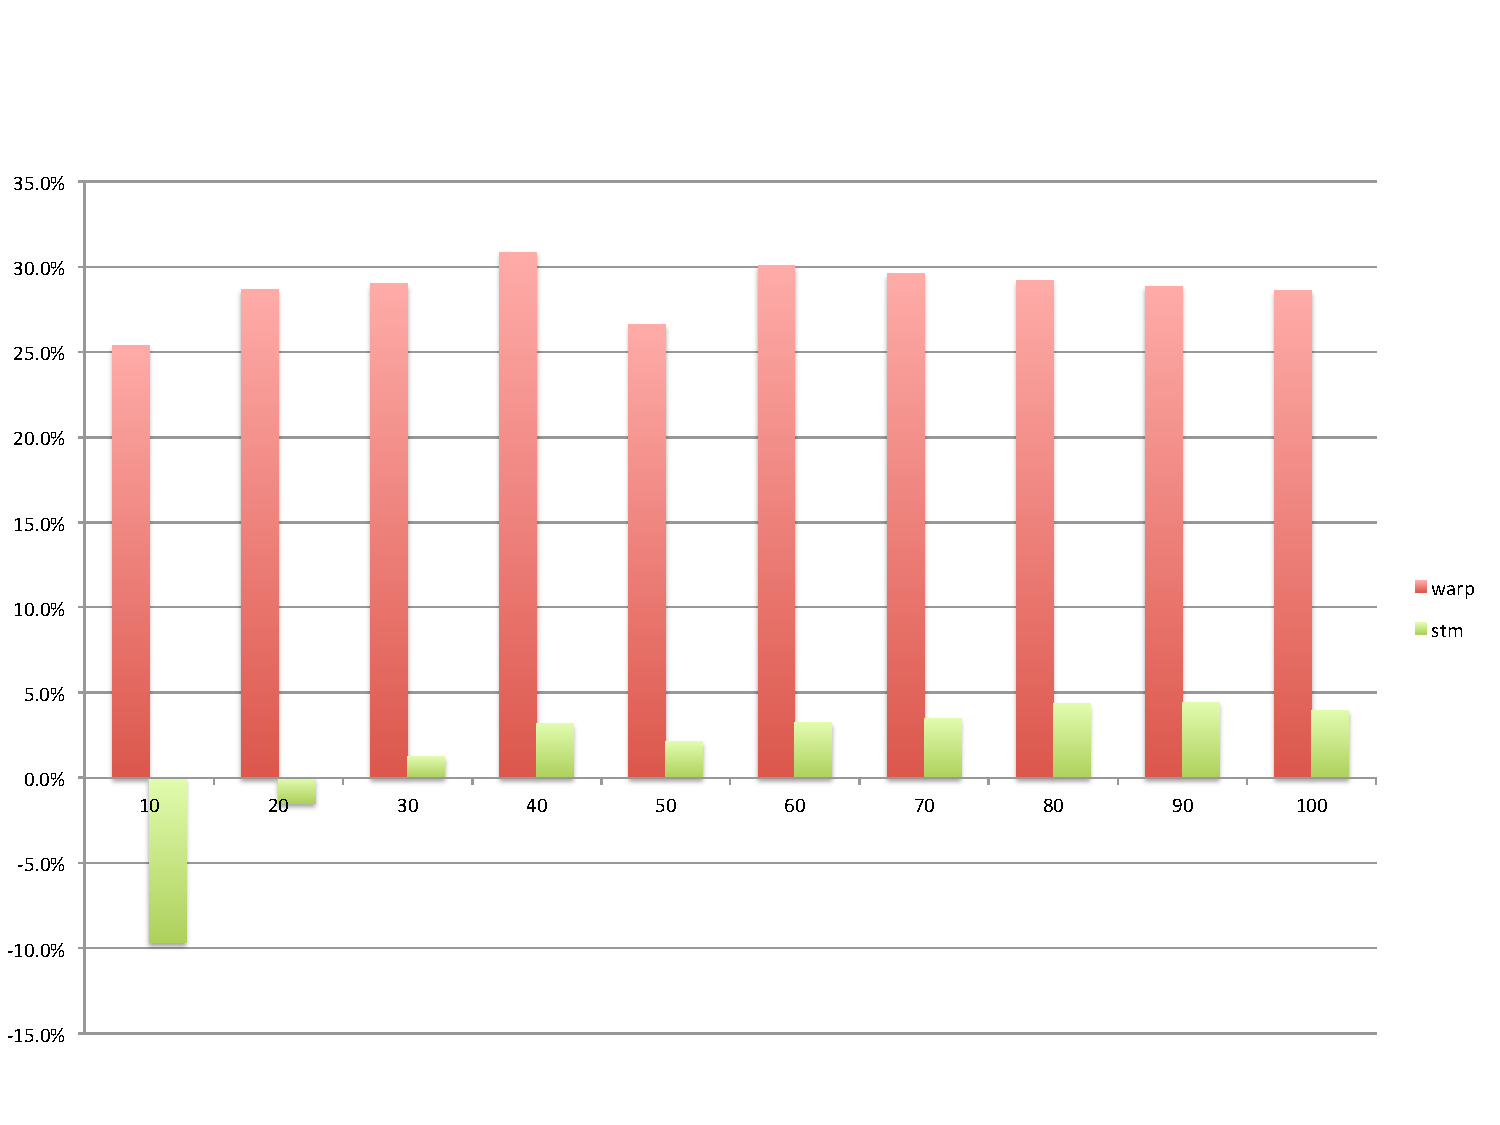
\includegraphics[width=\textwidth]{../../eval/32threads/case1it.pdf}
%		\caption{\label{Fi:case1th}Apache Tomcat {\sf ApplicationContext}: workload}
%	\end{minipage}
%	\hspace{0.05 \textwidth}
%	\begin{minipage}{0.3 \textwidth}
%		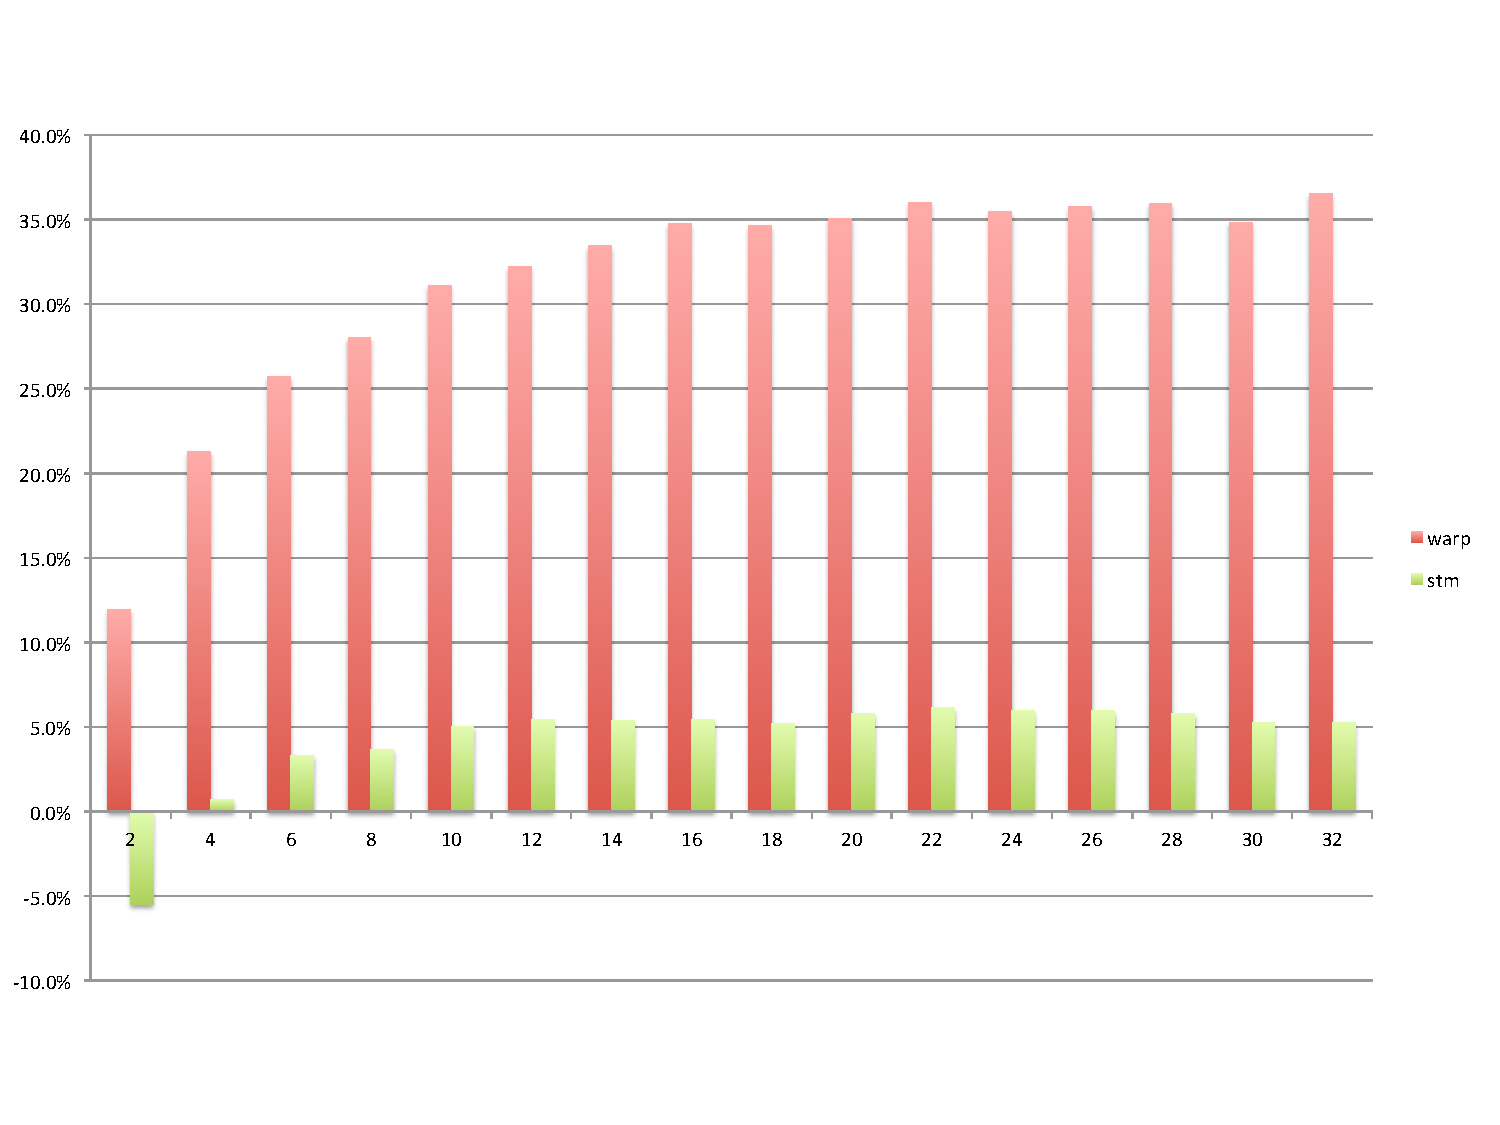
\includegraphics[width=\textwidth]{../../eval/32threads/case1th.pdf}
%		\caption{\label{Fi:case1th}Apache Tomcat {\sf ApplicationContext}: concurrency}
%	\end{minipage}
%	\hspace{0.05 \textwidth}
%	\begin{minipage}{0.3 \textwidth}
%		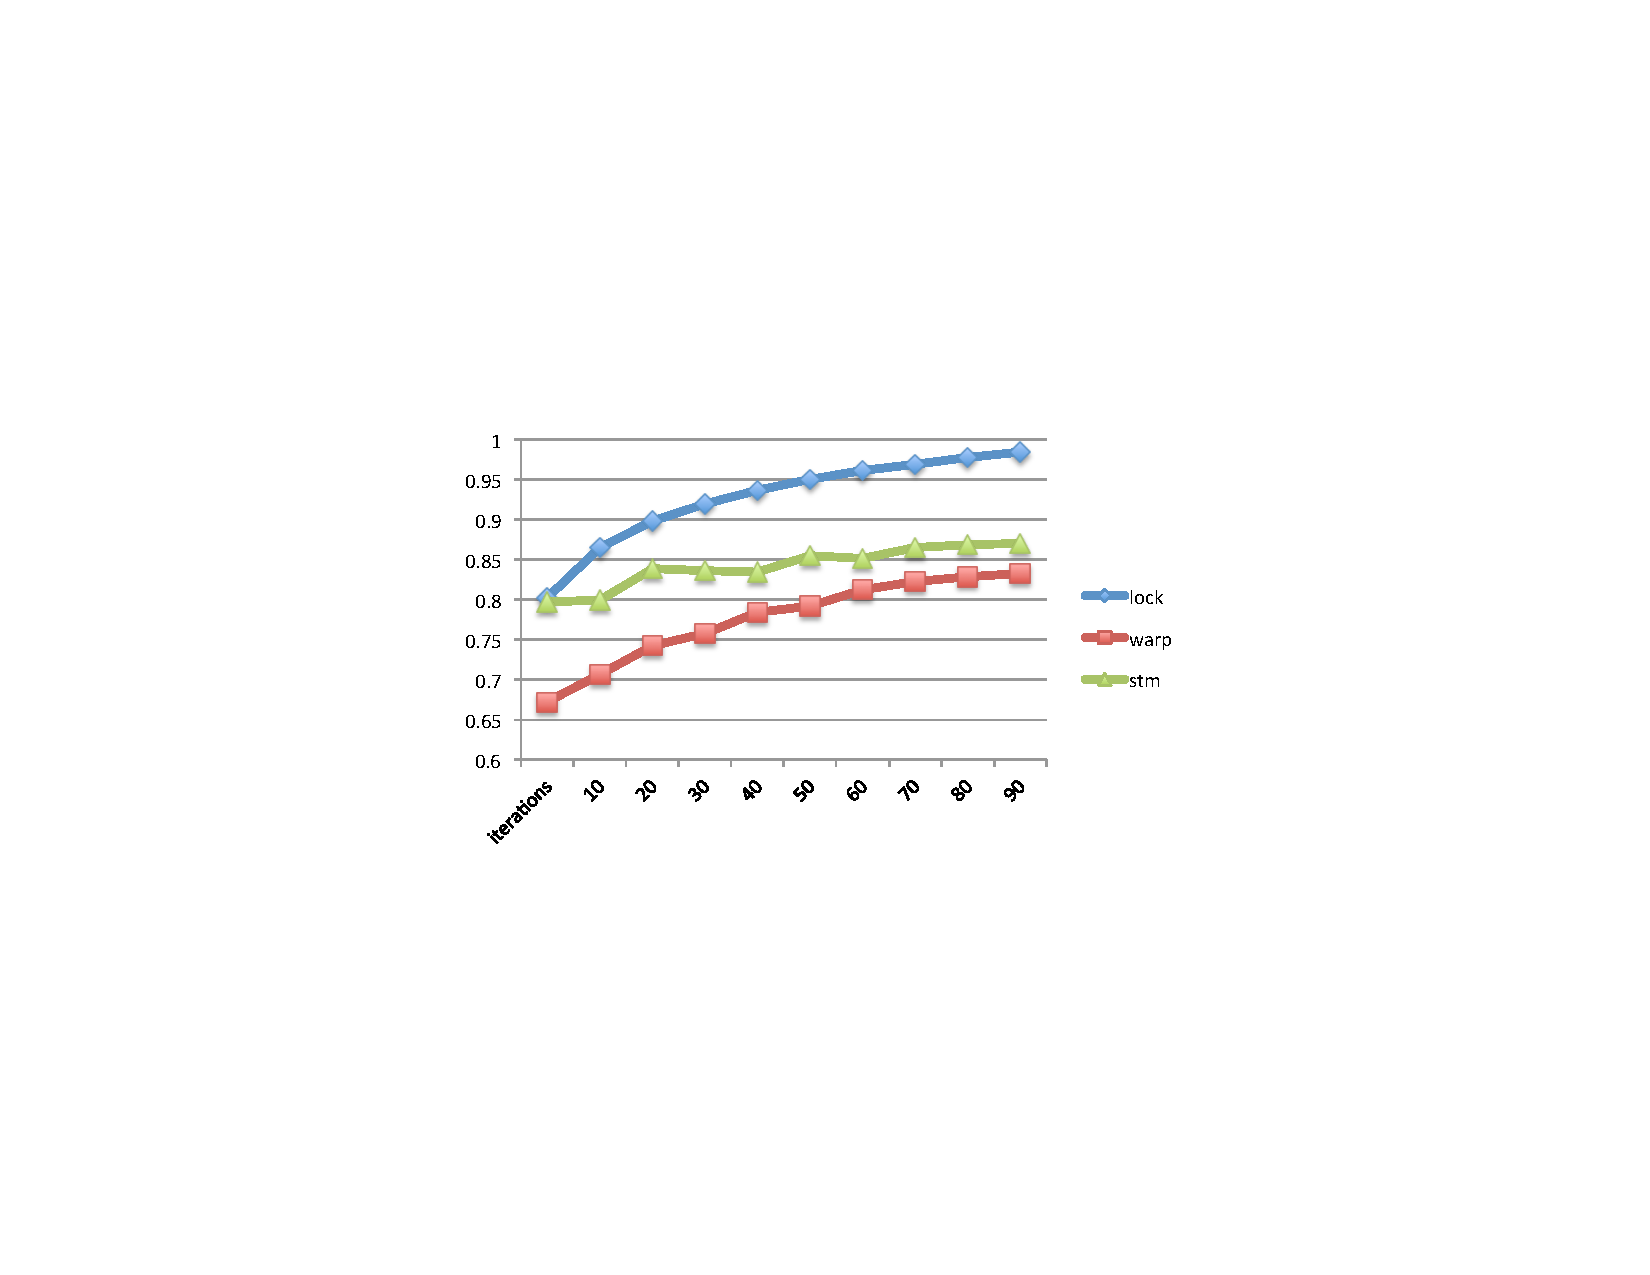
\includegraphics[width=\textwidth]{../../eval/32threads/case2it.pdf}
%		\caption{\label{Fi:case2it}dyuproject {\sf StandardConvertorCache}: workload}
%	\end{minipage}
%	\begin{minipage}{0.3 \textwidth}
%		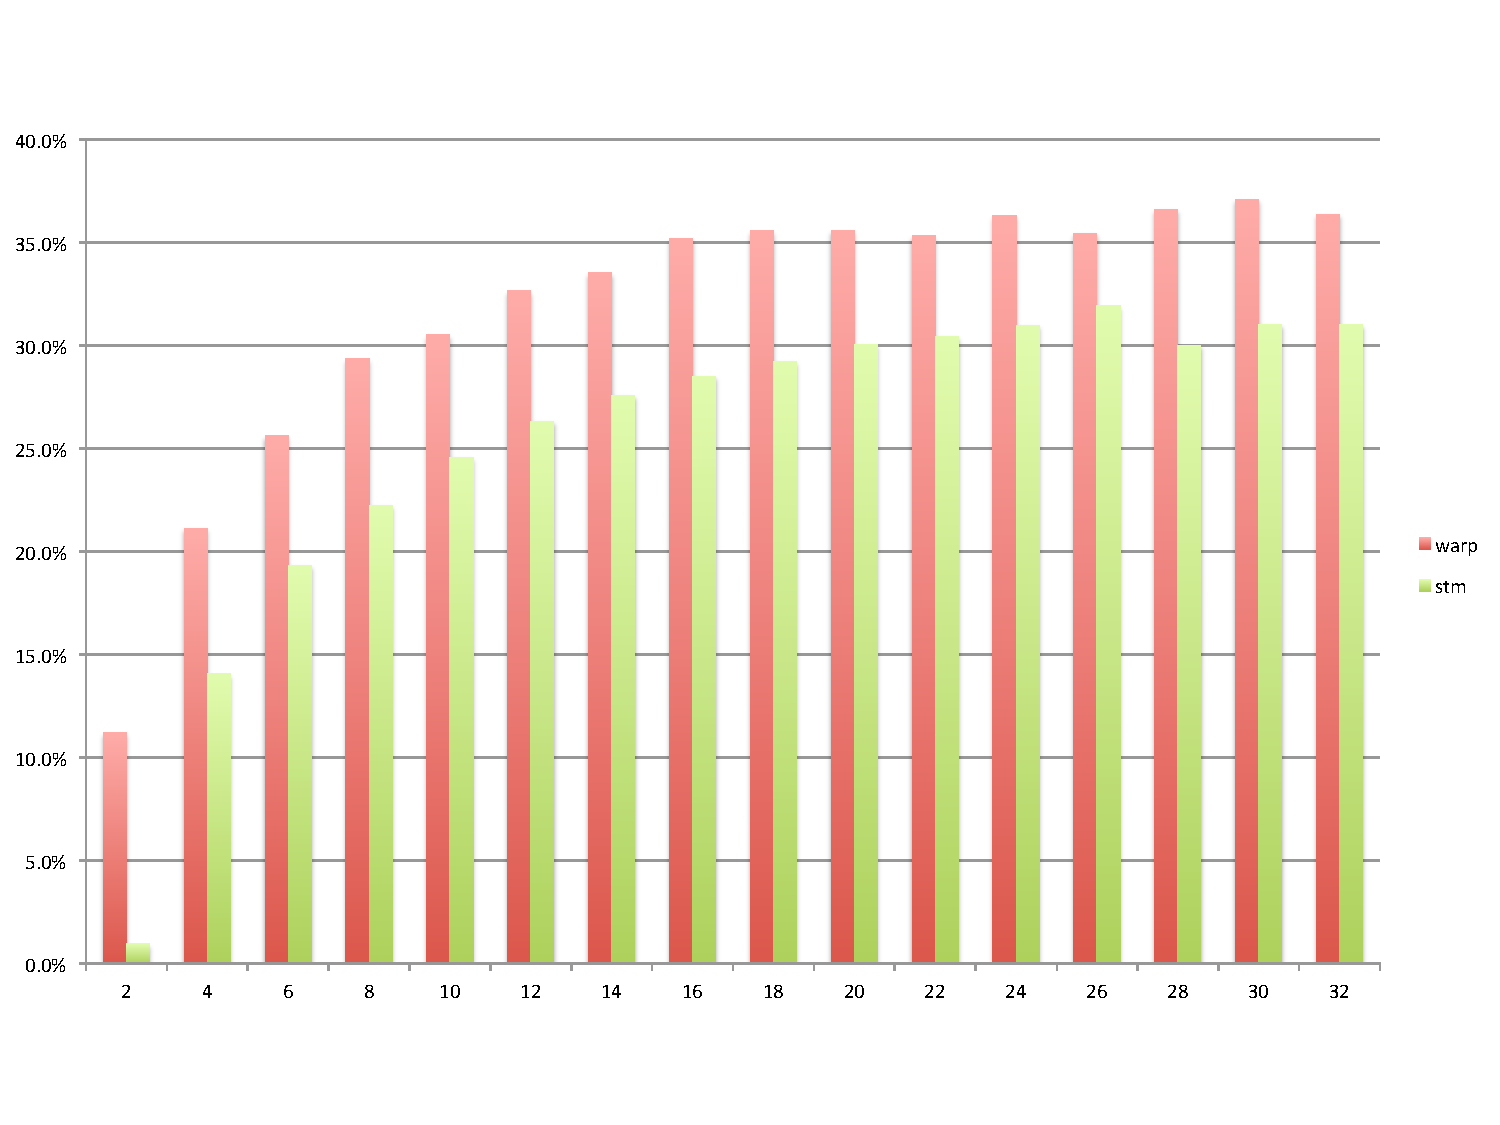
\includegraphics[width=\textwidth]{../../eval/32threads/case2th.pdf}
%		\caption{\label{Fi:case2th}dyuproject {\sf StandardConvertorCache}: concurrency}
%	\end{minipage}
%	\hspace{0.05 \textwidth}
%	\begin{minipage}{0.3 \textwidth}
%		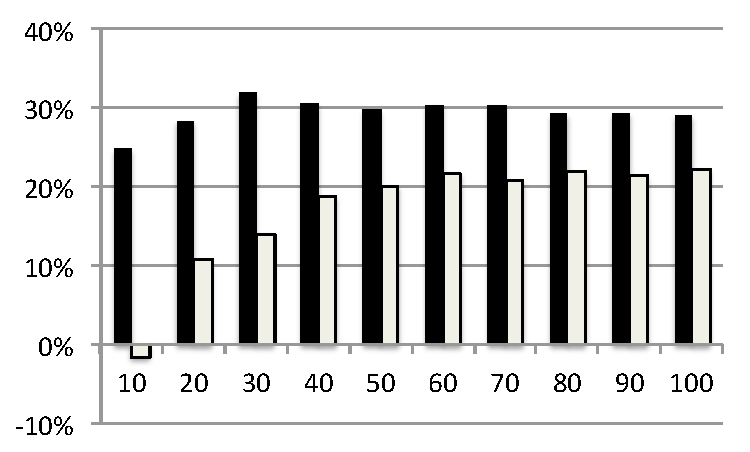
\includegraphics[width=\textwidth]{../../eval/32threads/case3it.pdf}
%		\caption{\label{Fi:case3it}Flexive {\sf FxValueRendererFactory}: workload}
%	\end{minipage}
%	\hspace{0.05 \textwidth}
%	\begin{minipage}{0.3 \textwidth}
%		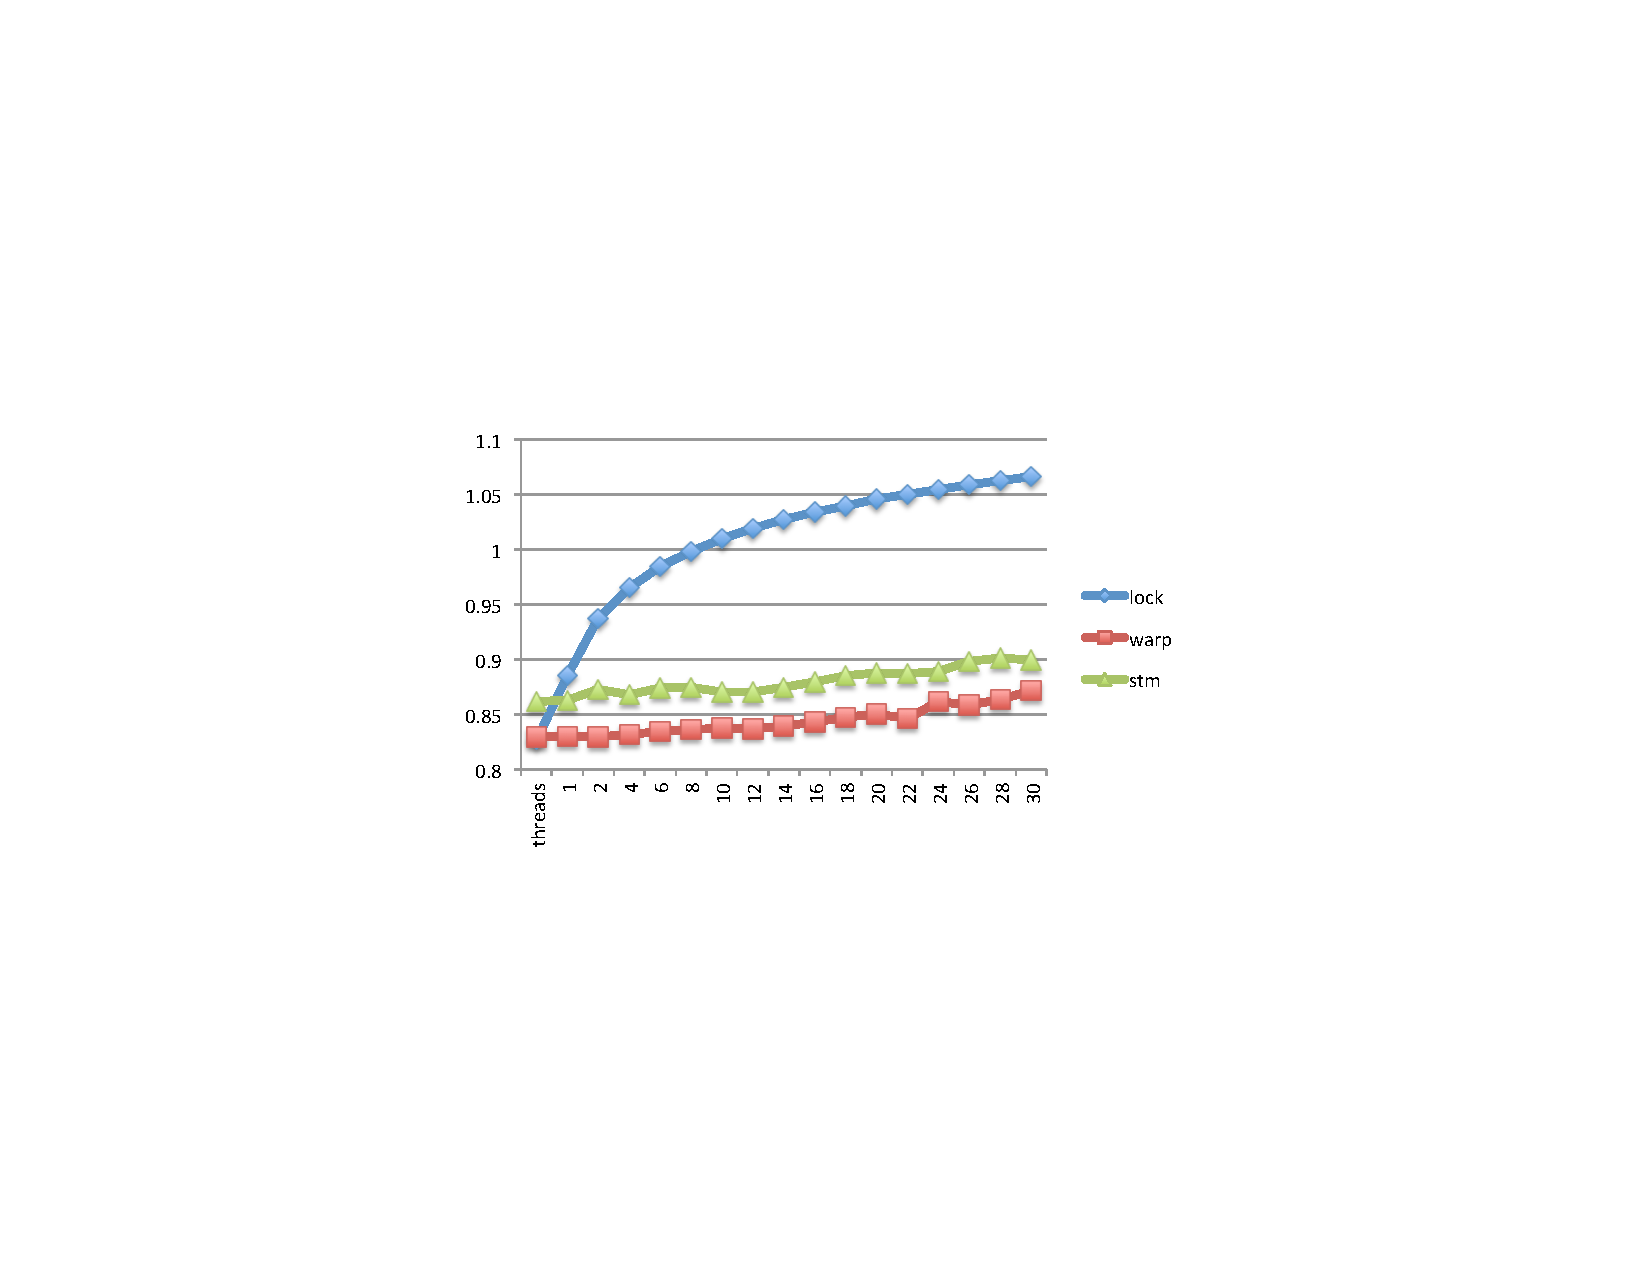
\includegraphics[width=\textwidth]{../../eval/32threads/case3th.pdf}
%		\caption{\label{Fi:case3th}Flexive {\sf FxValueRendererFactory}: concurrency}
%	\end{minipage}
%	\begin{minipage}{0.15 \textwidth}
%		\ 
%	\end{minipage}
%	\begin{minipage}{0.3 \textwidth}
%		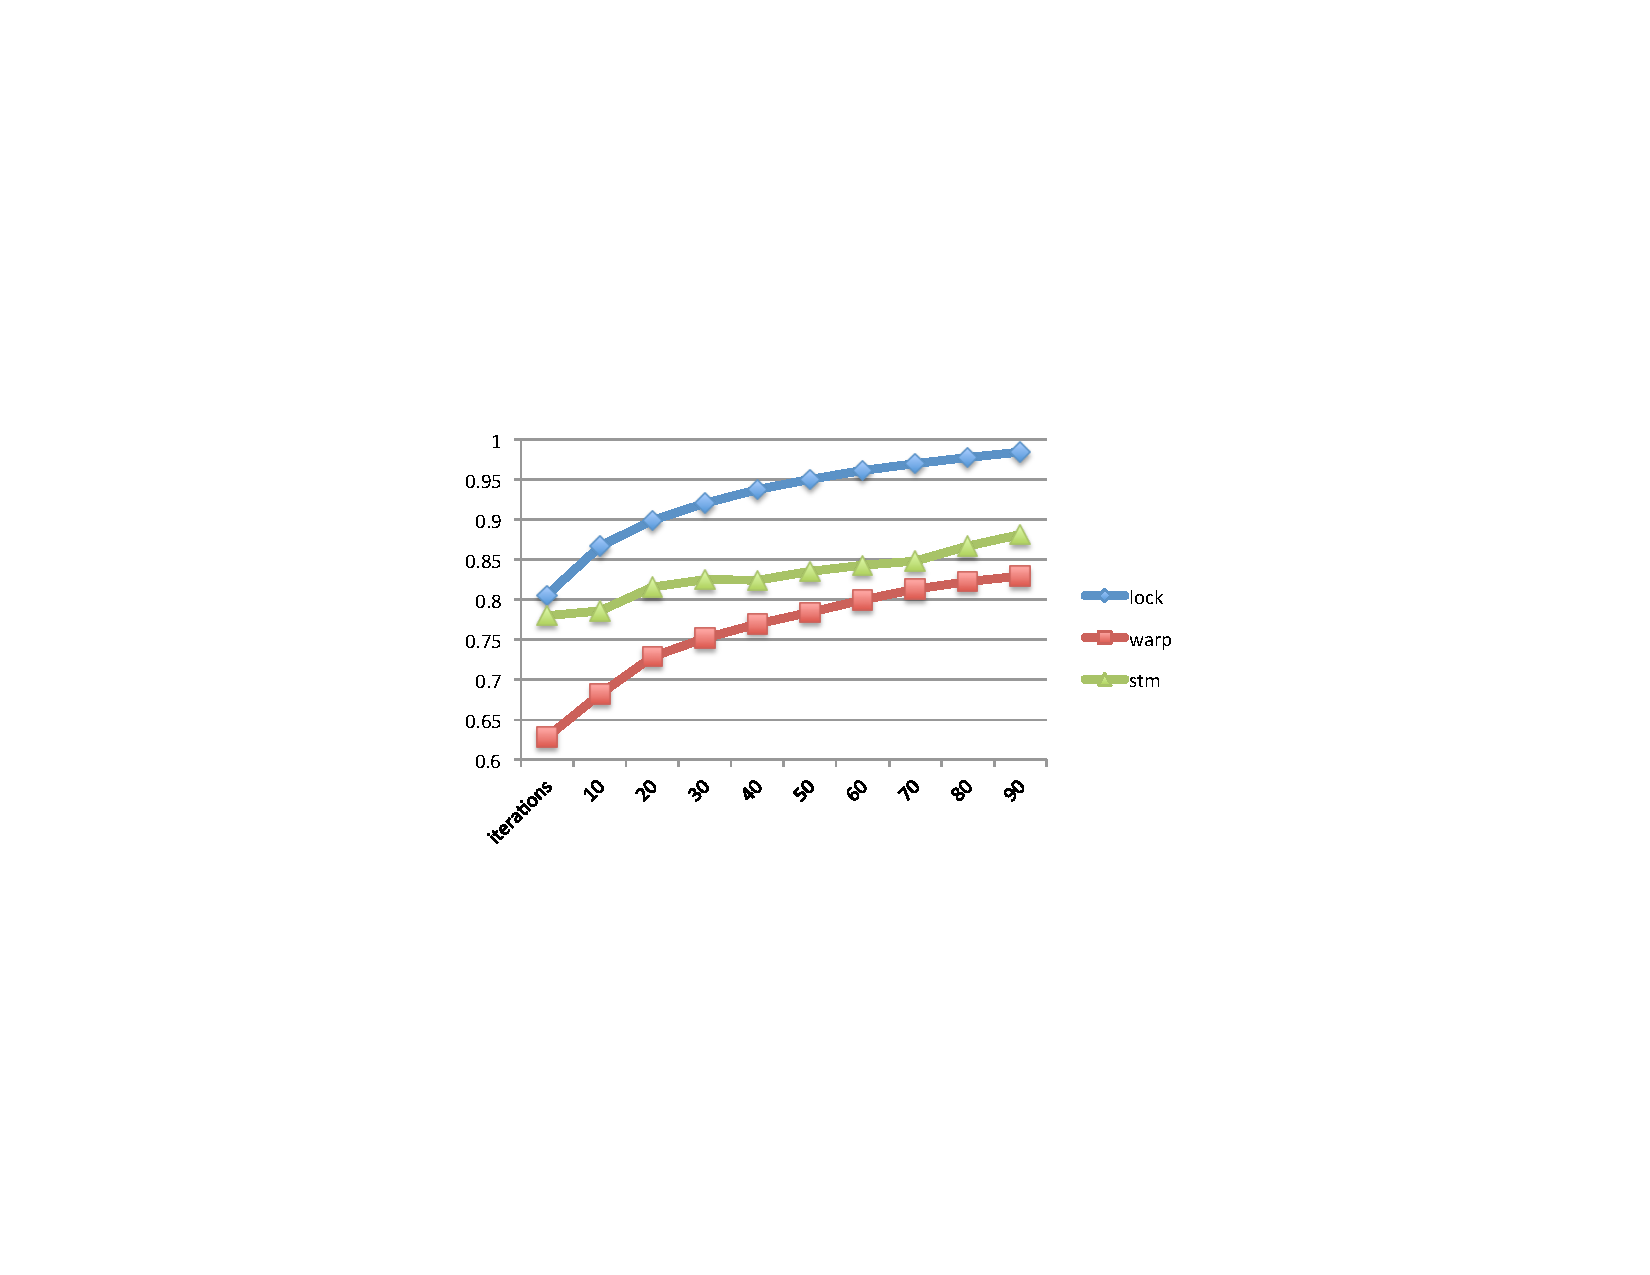
\includegraphics[width=\textwidth]{../../eval/32threads/case4it.pdf}
%		\caption{\label{Fi:case4it}Gridkit {\sf ReflectionPofSerializer}: workload}
%	\end{minipage}
%	\hspace{0.1 \textwidth}
%	\begin{minipage}{0.3 \textwidth}
%		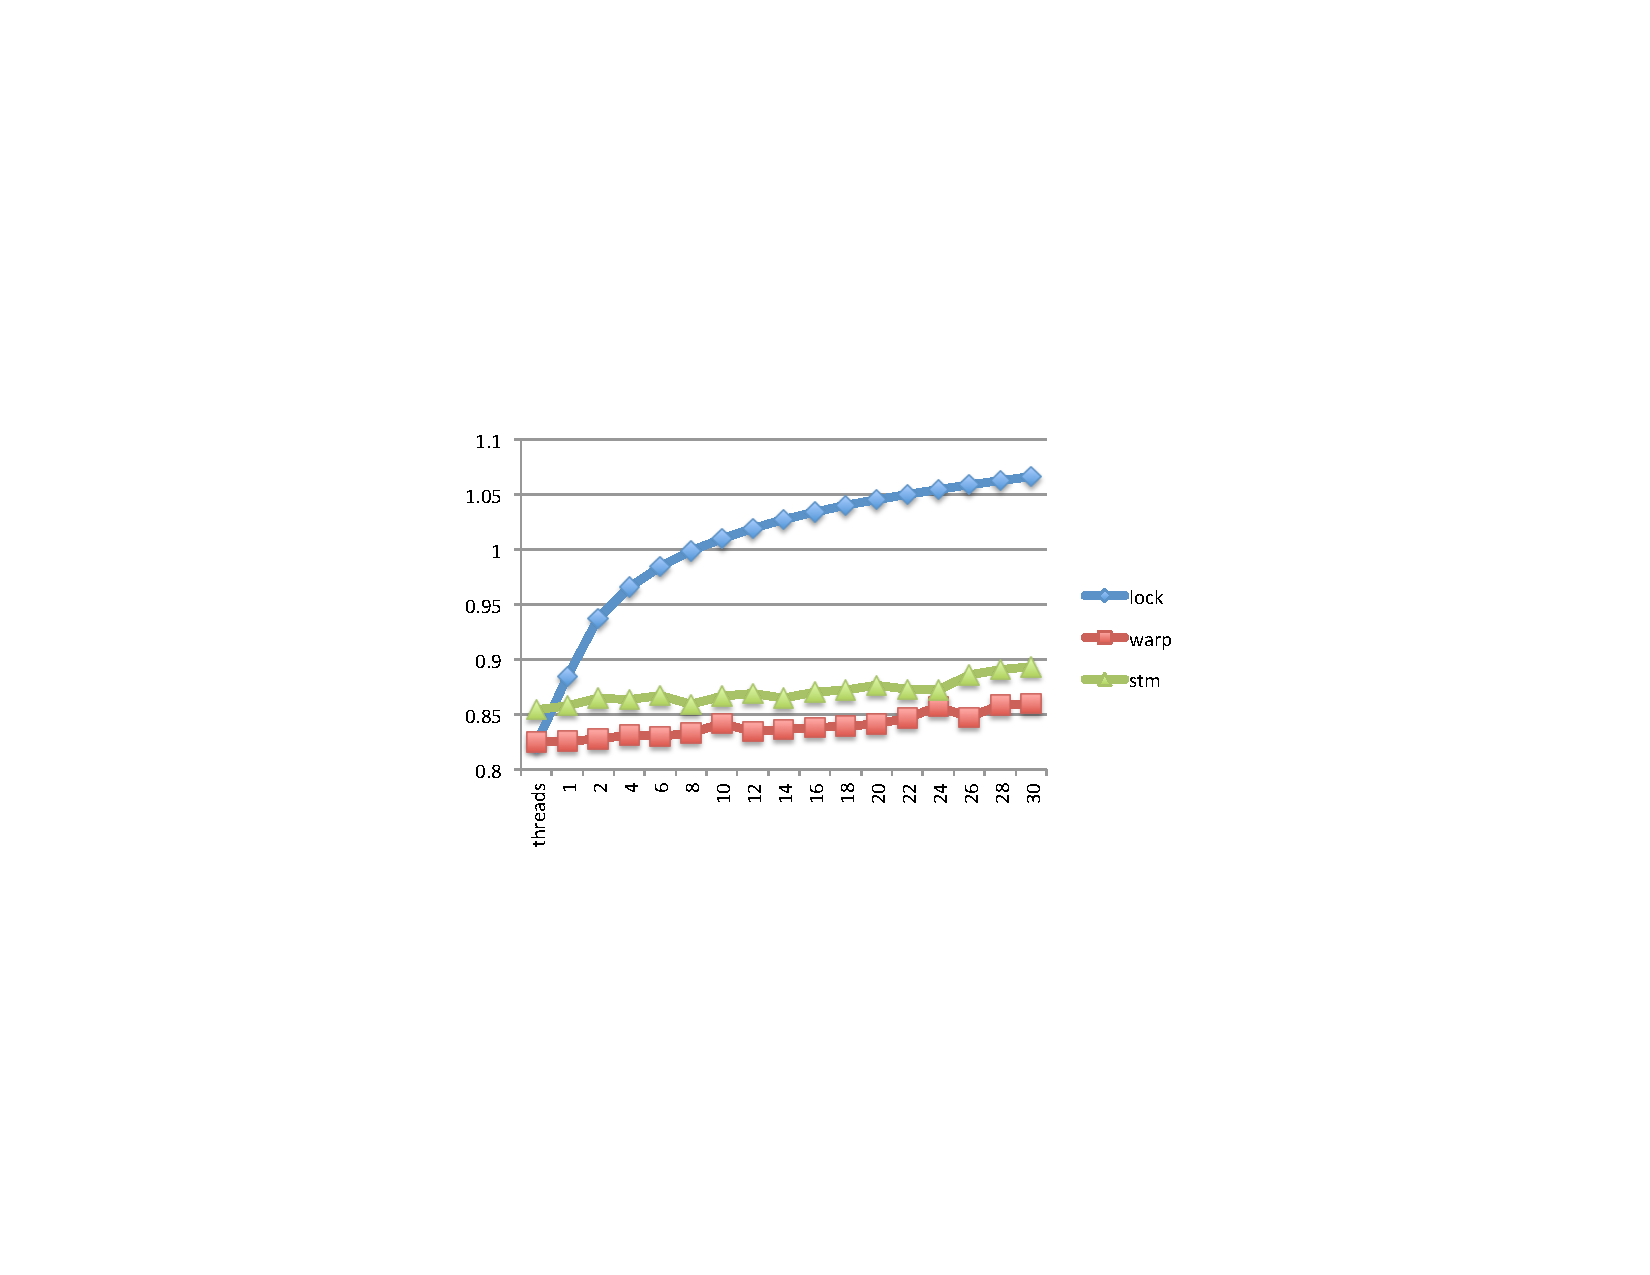
\includegraphics[width=\textwidth]{../../eval/32threads/case4th.pdf}
%		\caption{\label{Fi:case4th}Gridkit {\sf ReflectionPofSerializer}: concurrency}
%	\end{minipage}
%\end{figure*}

\vfill
